\section{Tipos en Java}
  Veamos ahora uno de los aspectos más importantes de la programación en \textit{Java}, sobre todo
  viniendo de algún otro lenguaje de programación.
  \textit{Java} es un lenguaje con tipos estáticos y fuertemente tipado, estos conceptos los 
  entenderemos mejor viendo algunos ejemplos.

  Primero tenemos que repasar el concepto de tipo.
  Todas las variables de un programa \textbf{tienen} un tipo definido, esto es importante ya que
  de esto dependerá la memoria que se necesite alocar para que la aplicación funcione.
  Ahora, si bien todas las variables tienen tipo, no siempre será el trabajo del programador
  definir el tipo de cada variable; aquí diferenciamos en dos sistemas de tipado:

  \begin{itemize}
    \item \textbf{Tipado estático:} El tipo de todas las variables es chequeado al compilar el 
      programa (i.e. antes de ejecutar).
      Esto tiene varias consecuencias, entre ellas, los tipos de las variables se definen junto
      a la variable\footnote{Dependiendo del lenguaje y del contexto puede que se necesite 
      declarar explícitamente el tipo de las variables} y que una vez que se define el tipo de
      una variable este no puede cambiar.
      Algunos ejemplos de lenguajes con tipado estático son \textit{Java}, \textit{C} y 
      \textit{Kotlin}.
    \item \textbf{Tipado dinámico:} El tipo de las variables se decide en tiempo de ejecución 
      (i.e. cuando la aplicación está corriendo).
      Contrario al tipado estático, como los tipos de las variables no se chequean en un 
      comienzo, no se tiene información sobre las variables hasta que son utilizadas, esto 
      implica que una variable puede \enquote{cambiar su tipo} durante la ejecución.
      Algunos ejemplos de lenguajes con tipado dinámico serían \textit{Python}, \textit{Ruby} y
      \textit{Javascript}.
  \end{itemize}
  
  Adicionalmente, también existen algunos lenguajes con \textit{tipado mixto}, esto quiere decir
  que se pueden definir algunas variables con tipo estático y otras con tipo dinámico.

  Por otro lado, existe el concepto de tipados fuerte y débil, es común que se confundan con las
  dos maneras de tipado que explicamos recién, pero son conceptos independientes entre sí.
  Más en detalle:

  \begin{itemize}
    \item \textbf{Tipado fuerte:} El programa exige \textit{seguridad de tipos}, esto significa 
      que una variable de tipo \textit{A} necesariamente se utilizará como si fuera de ese tipo
      y, en caso de que eso no se cumpla, se arrojará un error señalando que hubo un error de 
      tipo.
      Noten que esto no se ve afectado si el lenguaje es estático o dinámico ya que en ambos 
      casos el programa puede arrojar un error si hay un error de tipo.
      Ejemplos de esta modalidad de tipado son lenguajes como \textit{Java}, \textit{Kotlin} y
      \textit{Python}.
    \item \textbf{Tipado débil:} No existe garantía acerca de cómo utilizar cada tipo de 
      variable.
      Un caso típico en el que se ve este comportamiento es en lenguajes que utilizan punteros 
      (por ejemplo \textit{C}), ya que estos permiten manejar las variables apuntando a su 
      dirección de memoria ignorando el tipo de valor almacenado en esa dirección.\footnote{En 
      \textit{C} esto se puede apreciar en el uso de
      \href{https://www.tutorialspoint.com/cprogramming/c_pointer_arithmetic.htm}{aritmética de 
      punteros}.}
  \end{itemize}

  La mayoría de los lenguajes modernos aseguran la \textit{seguridad de tipos}, pero algunos 
  lenguajes más antiguos que siguen ocupándose frecuentemente en la actualidad son de tipado 
  débil (principalmente \textit{C} y \textit{Assembly}).

  Veamos cómo se ve reflejado esto en \textit{Java}.
  Para correr los ejemplos utilizaremos la consola interactiva de \textit{Java}, para esto ejecuten
  el comando \texttt{jshell} en la terminal.

  La sintaxis para definir una variable en java es \texttt{<type> <id> = <value>}, por ejemplo, si
  queremos definir una variable que almacene un entero entonces lo podemos hacer como:

  \begin{minted}{java}
    int i = 8000;
  \end{minted}

  Aquí es importante notar que en \textit{Java} \textbf{todas} las instrucciones deben terminar con
  un \texttt{;}.
  Luego, podemos modificar libremente el valor de \texttt{i} a otro entero (por ejemplo hacer 
  \texttt{i = 420}), pero no podemos asignarle un valor de un tipo distinto (e.g. \texttt{6.9}) 
  debido al tipado estático.

  \begin{exercise}
    Si un lenguaje de programación infiere el tipo de las variables por contexto, entonces el 
    lenguaje tiene tipado dinámico.
    ¿Es esto correcto?
  \end{exercise}

  \begin{exercise}
    ¿Por qué usarían un lenguaje estático?
    ¿Por qué usarían uno dinámico?
  \end{exercise}

  \begin{exercise}
    ¿Qué caso de uso podría tener un lenguaje de tipado débil?
  \end{exercise}

  \begin{exercise}
    En \textit{Perl} se pueden operar algunos valores de distinto tipo como si fueran el mismo,
    por ejemplo, el siguiente código entrega como resultado \mintinline{java}{42}:
    \begin{minted}{perl}
      $a = 11;
      $b = "31a";
      $c = $a + $b;
      print $c;
    \end{minted}

    ¿Qué clase de tipado se ve en el ejemplo?
  \end{exercise}
  
  \begin{exercise}
    En \textit{Kotlin} existe el tipo \mintinline{kotlin}{Any} que representa a todos los tipos, 
    esto significa que podemos asignarle cualquier valor a una variable definida con ese tipo, por
    ejemplo:

    \begin{minted}{kotlin}
      var a: Any = 0
      a = "Ola ceamos hamigos"
    \end{minted}

    Esto podría interpretarse como que \textit{Kotlin} tiene tipado dinámico, pero no es así.
    ¿Por qué el supertipo \mintinline{kotlin}{Any} no es un ejemplo de tipado dinámico?
  \end{exercise}

  \begin{exercise}
    En \textit{Javascript} existe lo que suele llamarse \textit{unholy trinity}.
    En términos simples, se puede entender como en la figura \ref{fig:unholy}.
    En código tendríamos lo siguiente:
    \begin{minted}{javascript}
      > false == [] 
        true
      > false == "0"
        true
      > [] == "0"
        false
    \end{minted}

    ¿Qué clase de tipado ejemplifica esto?
  \end{exercise}

  \begin{figure}[ht!]
    \centering
    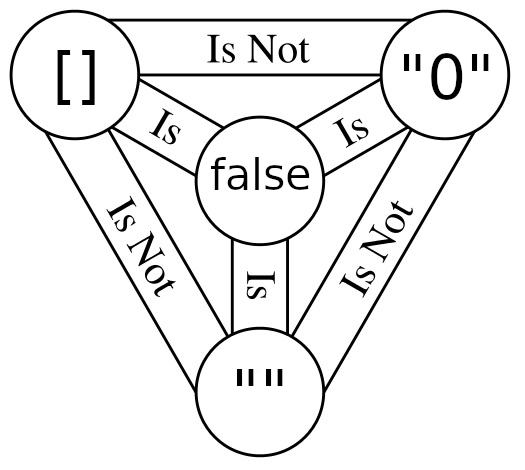
\includegraphics[width=0.5\textwidth]{Por algo se empieza/unholy.png}
    \caption{\textit{Unholy trinity}}
    \label{fig:unholy}
  \end{figure}

  \subimport{Tipos_en_Java/}{Inferencia_de_tipos.tex}